\documentclass[8pt, xcolor={svgnames}, hyperref={colorlinks, linkcolor=black, citecolor=amethyst, urlcolor=amethyst}]{beamer}


\usepackage[labelfont={color=amethyst,bf}]{caption}
\usetheme[progressbar=frametitle]{metropolis}
\usepackage{appendixnumberbeamer}
\usepackage{url}
\usepackage{booktabs}
\usepackage{braket}
\usepackage[scale=2]{ccicons}
\usepackage{amsfonts} 
\usepackage{amssymb}
\usepackage[english]{babel}
\colorlet{col1}{teal}
\colorlet{col2}{yellow}
\colorlet{col3}{green}
\usepackage{fontawesome}
\usepackage{subcaption}
\usepackage{multicol}
\usepackage{bm}
\usepackage{algorithm}
\usepackage{algpseudocode}
\usepackage{enumitem}

\usepackage[]{pseudo}


\usepackage{tikz}
\usetikzlibrary{positioning,arrows,calc,math,angles,quotes}
\usepackage{blochsphere}

\usetikzlibrary{arrows,automata}
\usetikzlibrary{positioning}
\usetikzlibrary{arrows.meta,
                bending,
                intersections,
                quotes,
                shapes.geometric}

\tikzset{
    state/.style={
           rectangle,
           rounded corners,
           draw=black, very thick,
           minimum height=1em,
           inner sep=2pt,
           text centered,
           },
}




\definecolor{myv}{rgb}{0.36, 0.22, 0.33}
\definecolor{gio}{rgb}{0.45, 0.31, 0.59}
\definecolor{light}{rgb}{0.8, 0.8, 1}
\definecolor{warmblack}{rgb}{0.0, 0.26, 0.26}
\definecolor{brown(web)}{rgb}{0.65, 0.16, 0.16}
\definecolor{cadmiumgreen}{rgb}{0.0, 0.42, 0.24}
\definecolor{darkmidnightblue}{rgb}{0.0, 0.2, 0.4}
\definecolor{brightube}{rgb}{0.82, 0.62, 0.91}

\definecolor{codegreen}{rgb}{0,0.6,0}
\definecolor{codegray}{rgb}{0.5,0.5,0.5}
\definecolor{codepurple}{rgb}{0.58,0,0.82}
\definecolor{backcolour}{rgb}{0.95,0.95,0.92}
\definecolor{amethyst}{rgb}{0.6, 0.33, 0.73}

\definecolor{light-gray}{gray}{0.95}
\newcommand{\code}[1]{\colorbox{light-gray}{\texttt{#1}}}
\usepackage{listings}
\lstdefinestyle{mystyle}{
    backgroundcolor=\color{backcolour},   
    commentstyle=\color{codegreen},
    keywordstyle=\color{codepurple},
    numberstyle=\tiny\color{codepurple},
    stringstyle=\color{magenta},
    basicstyle=\scriptsize,
    breakatwhitespace=false,         
    breaklines=true,                 
    captionpos=b,                    
    keepspaces=true,                 
    numbers=left,                    
    numbersep=5pt,                  
    showspaces=false,                
    showstringspaces=false,
    showtabs=false,                  
    tabsize=2
}

\lstset{style=mystyle}
\usepackage[most]{tcolorbox}
\usepackage{xcolor}

%\usepackage[citecolor = green, linkcolor = blue, bookmarks=true, urlcolor=blue,
%colorlinks=true, pagebackref=true]{hyperref}


%\usepackage{xspace}

\title{Doing full stack QML using \texttt{qibo}}
\date{24 May 2023}
\author[Matteo Robbiati]{Matteo Robbiati \textbf{\textcolor{amethyst}{feat.}} Alejandro Sopena}
\titlegraphic{
\begin{tikzpicture}[overlay, remember picture]

\node[at=(current page.south east), anchor=south east] {%
\includegraphics[width=.18\textwidth]{figures/qibo.png} 

\includegraphics[width=.18\textwidth]{figures/unimi.png} 
\includegraphics[width=.18\textwidth]{figures/cern.png}  
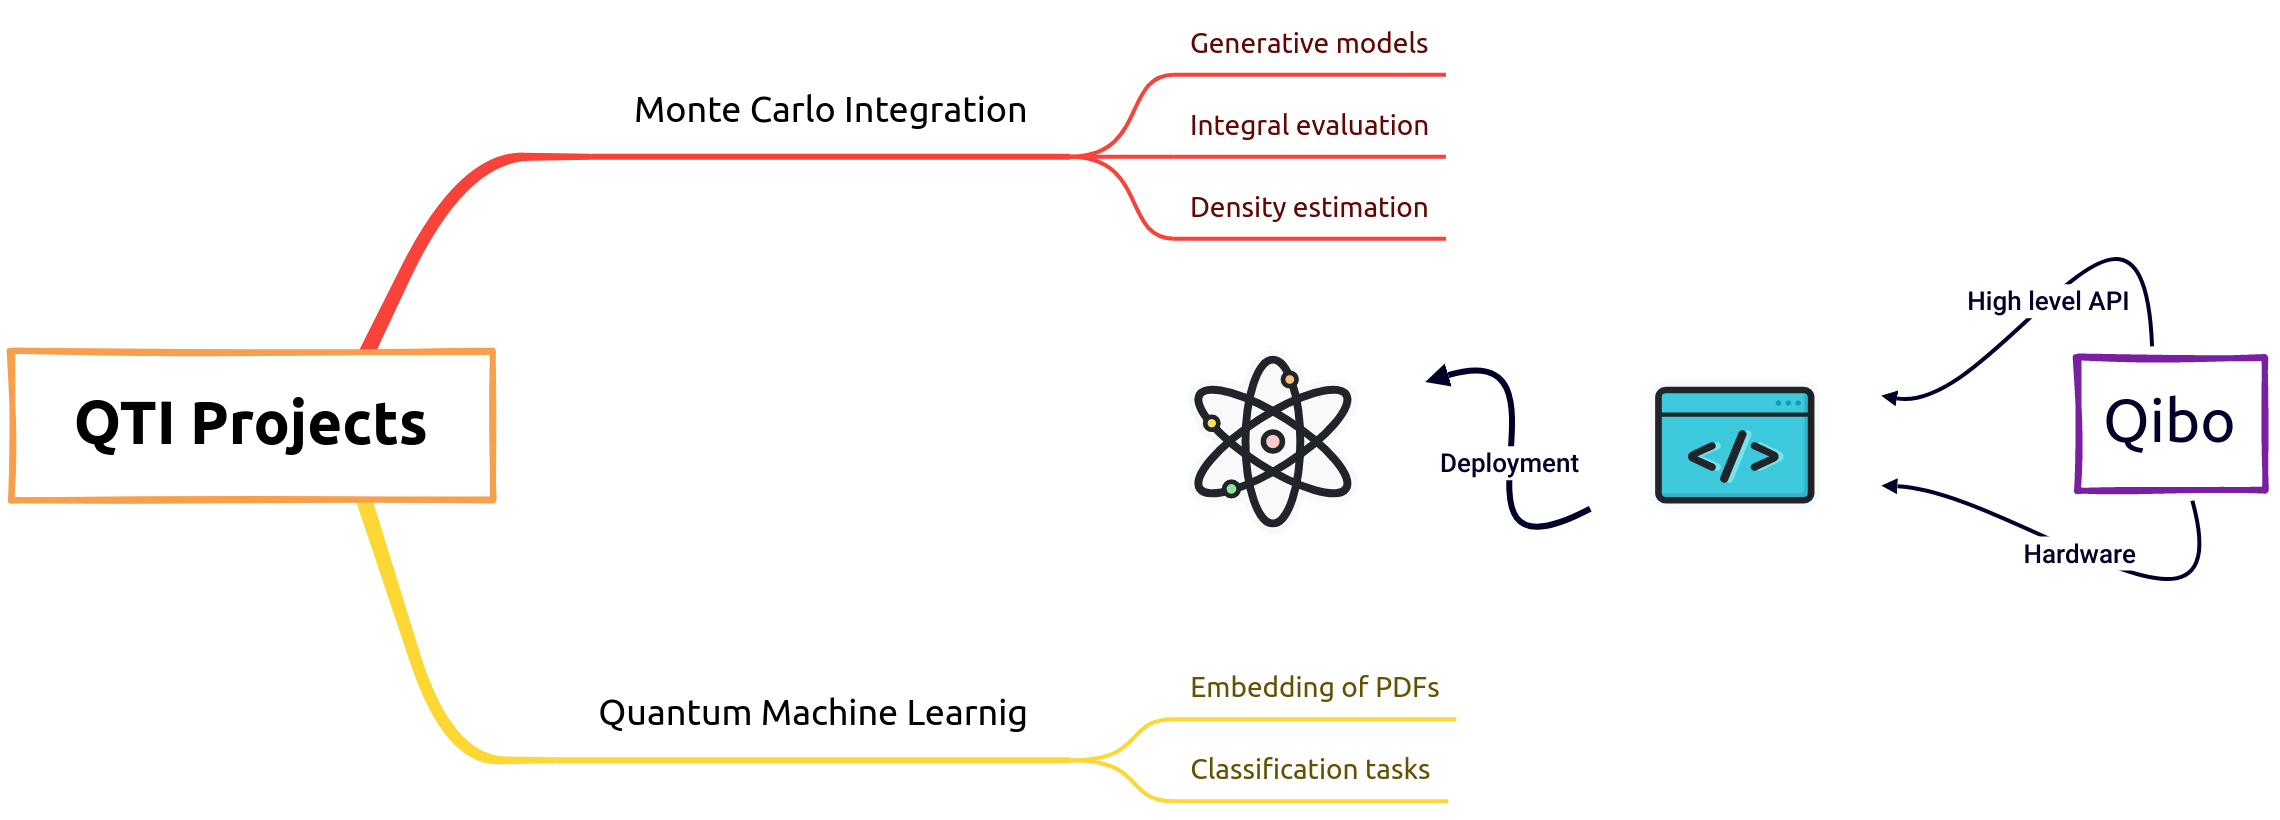
\includegraphics[width=.18\textwidth]{figures/qti.png}  
};
\end{tikzpicture}
}



\begin{document}


\maketitle

\begin{frame}{Working in the NISQ era}
    \begin{figure}  
    \includegraphics[width=1\textwidth]{figures/mr_research.png}
    \end{figure}
    \vspace{-0.5cm}
\end{frame}

\begin{frame}{The \texttt{qibo} ecosystem}
\small
    \begin{figure}  
    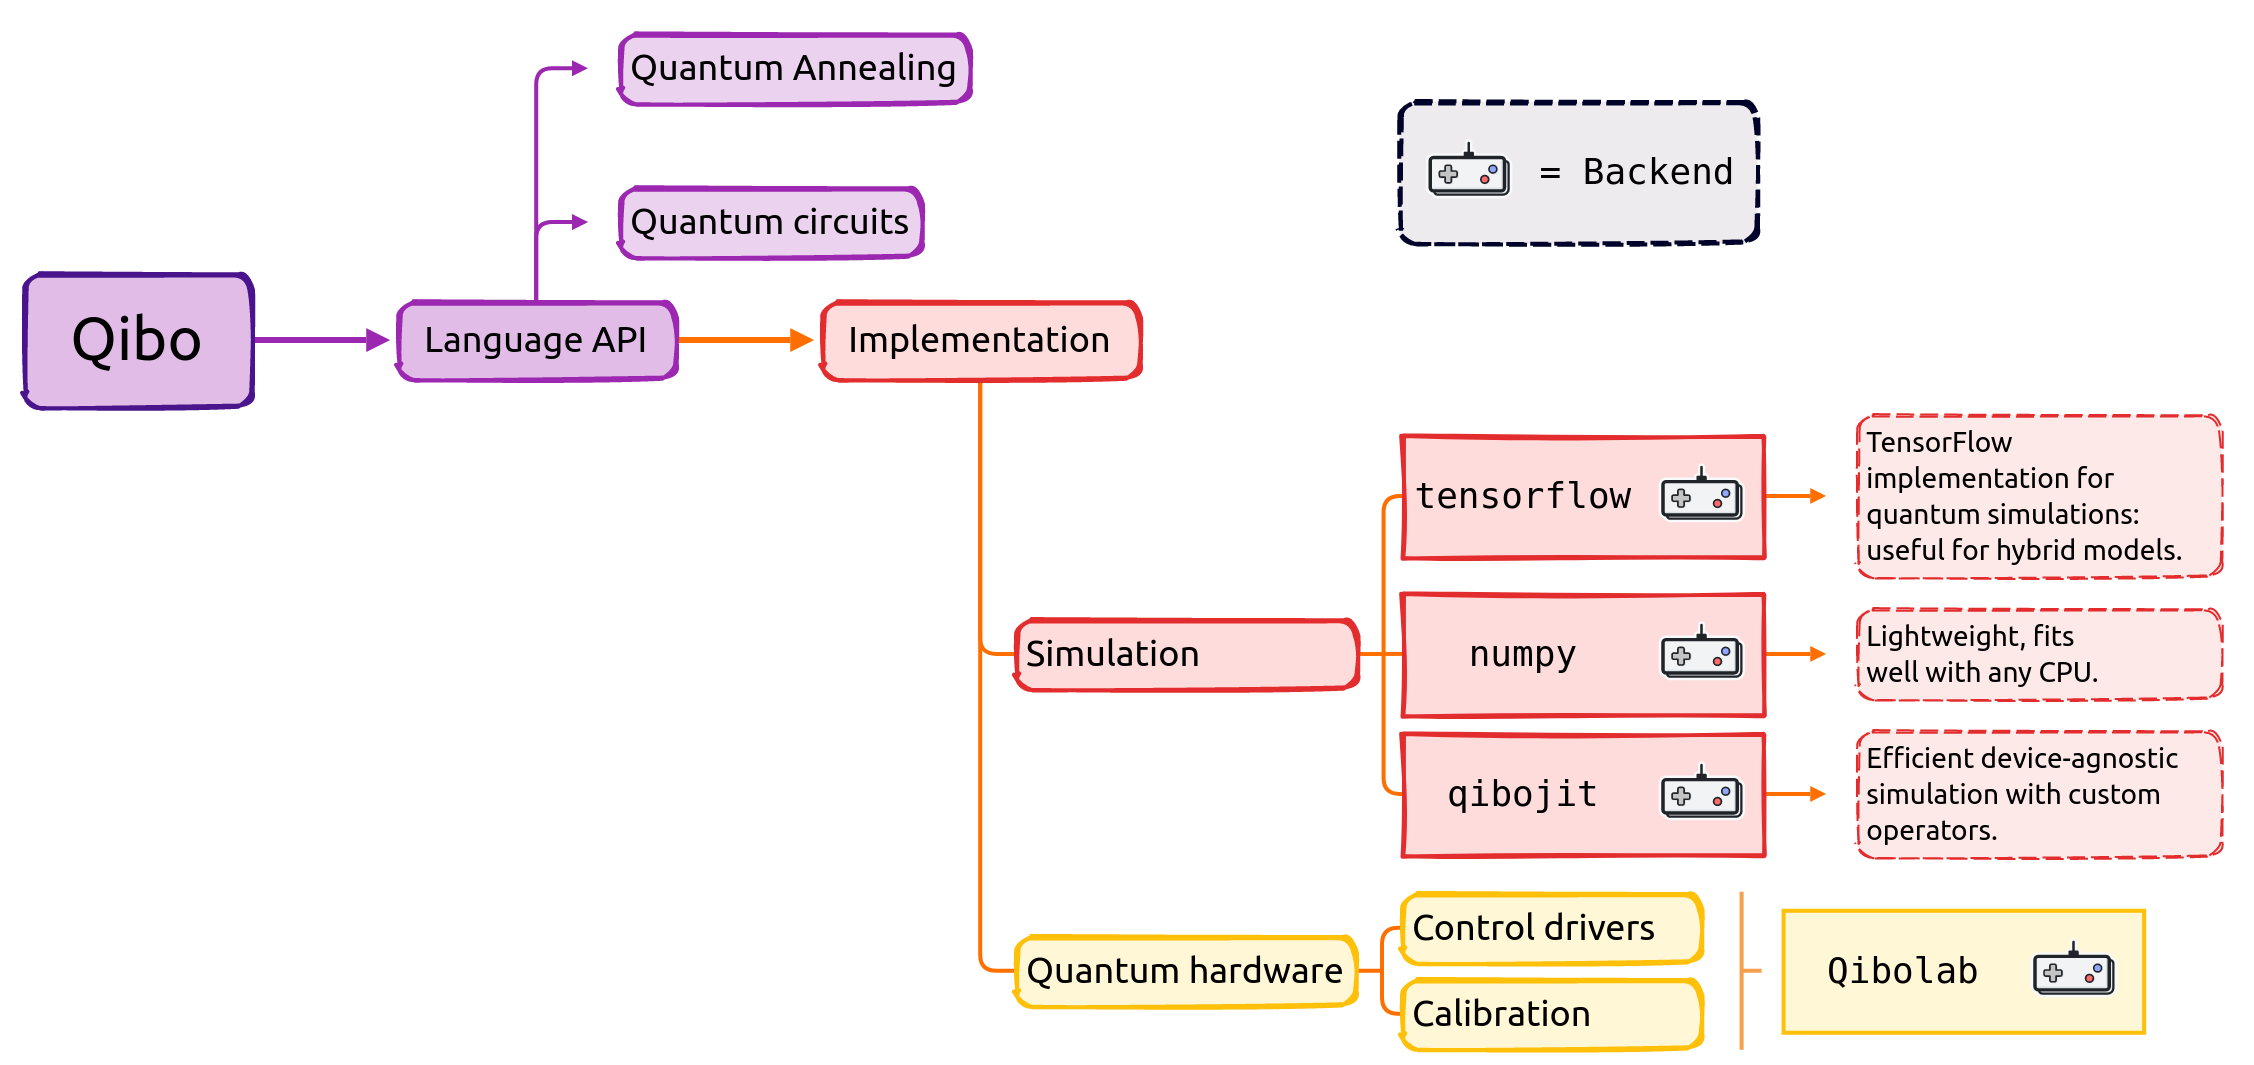
\includegraphics[width=1\textwidth]{figures/qibo_ecosystem.png}
    \end{figure}
\end{frame}

\section{Two snapshots}

\begin{frame}[fragile]{Adiabatic Evolution}
\faArrowCircleRight\,\, Consider two Hamiltonians $H_0$ and $H_1$, whose ground
states are $\ket{g_0}$ and $\ket{g_1}$.
\pause

\faArrowCircleRight\,\, We call Adiabatic Evolution the process represented by:
\pause

\begin{equation}
H_{ad}(\tau; \bm{\theta}) = \bigl[ 1 - s(\tau; \bm{\theta}) \bigr] H_0 +
s(\tau; \bm{\theta}) H_1.
\end{equation}
\pause

\faArrowCircleRight\,\, in which we parametrize the \textbf{scheduling} function $s$.
\pause

\begin{tcolorbox}[breakable, enhanced]
\begin{lstlisting}[language=Python]
    # with qibo we can implement an Adiabatic Evolution via trotter formula
    from qibo import models, hamiltonians, callbacks

    # problem's parameters
    nqubits = 1
    h0 = hamiltonians.X(nqubits)
    h1 = hamiltonians.Z(nqubits)
    target_observable = h1

    # we track the energy of h1 on the evolved ground state
    energies = callbacks.Energy(target_observable)
    evolution = models.AdiabaticEvolution(
        h0=h0, h1=h1, s = lambda t : t, dt=0.1, callbacks = [energies])

    # calculate the evolved final state at time t=final_time
    evolved_state = evolution(final_time = final_time)
\end{lstlisting}
\end{tcolorbox}

\end{frame}

% SLIDE UNO QML
\begin{frame}{Quantum Machine Learning - doing ML using QC}

\vspace{1.5cm}


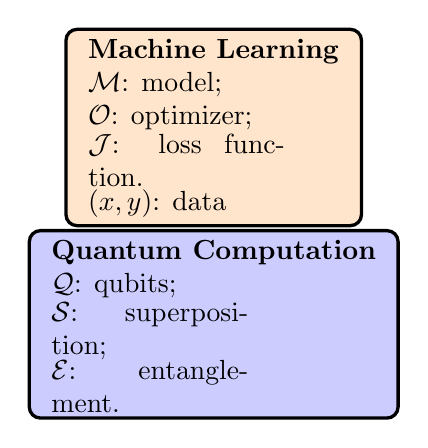
\begin{tikzpicture}[->,>=stealth']

 \node[state, fill=orange!20] (ML) 
 {\begin{tabular}{l}
 \textbf{Machine Learning}\\ 
 \parbox{2.5cm}{$\mathcal{M}$: model;}\\
 \parbox{2.5cm}{$\mathcal{O}$: optimizer;}\\
 \parbox{2.5cm}{$\mathcal{J}$: loss function.}\\
 \parbox{2.5cm}{$(x, y)$: data}
  \end{tabular}
  };
  
  \node[state,
  below of = ML,
  yshift=-1.5cm, fill=blue!20] (QC) 
 {\begin{tabular}{l}
 \textbf{Quantum Computation}\\ 
 \parbox{2.5cm}{$\mathcal{Q}$: qubits;} \\
 \parbox{2.5cm}{$\mathcal{S}$: superposition;}\\
 \parbox{2.5cm}{$\mathcal{E}$: entanglement.}
  \end{tabular}
  };
  
\end{tikzpicture}
\end{frame}


% SLIDE 2 QML
\begin{frame}{Quantum Machine Learning - operating on qubits}

\vspace{1.77cm}

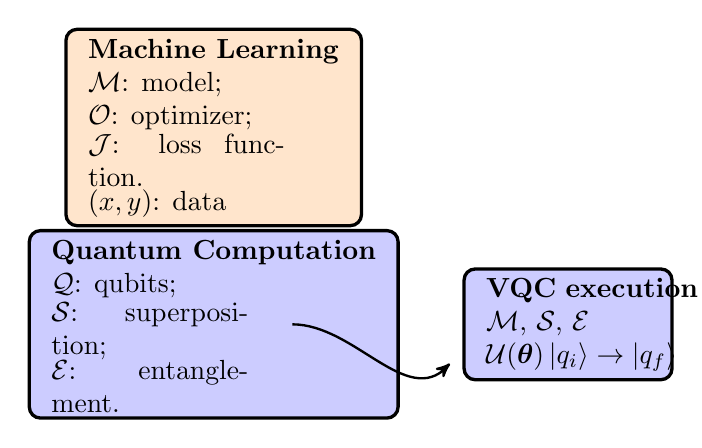
\begin{tikzpicture}[->,>=stealth']

 \node[state, fill=orange!20] (ML) 
 {\begin{tabular}{l}
 \textbf{Machine Learning}\\ 
 \parbox{2.5cm}{$\mathcal{M}$: model;}\\
 \parbox{2.5cm}{$\mathcal{O}$: optimizer;}\\
 \parbox{2.5cm}{$\mathcal{J}$: loss function.}\\
 \parbox{2.5cm}{$(x, y)$: data}
  \end{tabular}
  };
  
  \node[state,
  below of = ML,
  yshift=-1.5cm, fill=blue!20] (QC) 
 {\begin{tabular}{l}
 \textbf{Quantum Computation}\\ 
 \parbox{2.5cm}{$\mathcal{Q}$: qubits;} \\
 \parbox{2.5cm}{$\mathcal{S}$: superposition;}\\
 \parbox{2.5cm}{$\mathcal{E}$: entanglement.}
  \end{tabular}
  };
  
   \node[state,
    right of=QC,
    yshift=0cm,
    anchor=center,
    node distance=4.5cm, 	
    text width=2.5cm, fill=blue!20] (VQC) 
 {%
 \begin{tabular}{l}
  \textbf{VQC execution}\\
  $\mathcal{M}$, $\mathcal{S}$, $\mathcal{E}$ \\
  \parbox{2.8cm}{$\mathcal{U}(\bm{\theta})\ket{q_i} \to \ket{q_f}$}
 \end{tabular}
 };
 
  \draw[line width=0.3mm] (1, -2.5)  to[out=0, in=230] (3, -3);
\end{tikzpicture}

\end{frame}

% SLIDE 3 QML
\begin{frame}{Quantum Machine Learning - natural randomness}

\vspace{1.77cm}

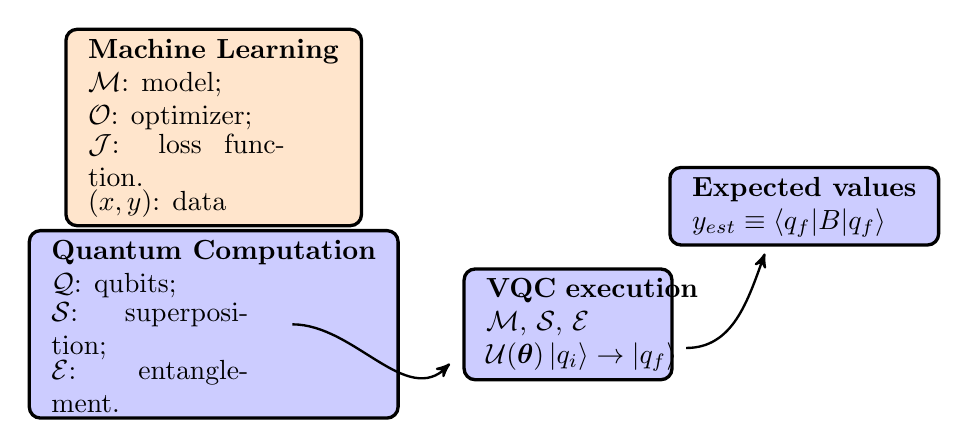
\begin{tikzpicture}[->,>=stealth']

 \node[state, fill=orange!20] (ML) 
 {\begin{tabular}{l}
 \textbf{Machine Learning}\\ 
 \parbox{2.5cm}{$\mathcal{M}$: model;}\\
 \parbox{2.5cm}{$\mathcal{O}$: optimizer;}\\
 \parbox{2.5cm}{$\mathcal{J}$: loss function.}\\
 \parbox{2.5cm}{$(x, y)$: data}
  \end{tabular}
  };
  
  \node[state,
  below of = ML,
  yshift=-1.5cm, fill=blue!20] (QC) 
 {\begin{tabular}{l}
 \textbf{Quantum Computation}\\ 
 \parbox{2.5cm}{$\mathcal{Q}$: qubits;} \\
 \parbox{2.5cm}{$\mathcal{S}$: superposition;}\\
 \parbox{2.5cm}{$\mathcal{E}$: entanglement.}
  \end{tabular}
  };
  
   \node[state,
    right of=QC,
    yshift=0cm,
    anchor=center,
    node distance=4.5cm, 	
    text width=2.5cm, fill=blue!20] (VQC) 
 {%
 \begin{tabular}{l}
  \textbf{VQC execution}\\
  $\mathcal{M}$, $\mathcal{S}$, $\mathcal{E}$ \\
  \parbox{2.8cm}{$\mathcal{U}(\bm{\theta})\ket{q_i} \to \ket{q_f}$}
 \end{tabular}
 };
 
\node[state,
  right of = VQC,
  node distance = 3cm,
  yshift=1.5cm, fill=blue!20] (NSHOT) 
 {\begin{tabular}{l}
 \textbf{Expected values}\\ 
 $y_{est} \equiv \braket{q_f|B|q_f}$
  \end{tabular}
  };
 
\draw[line width=0.3mm] (1, -2.5)  to[out=0, in=230] (3, -3);
\draw[line width=0.3mm] (6, -2.8)  to[out=0, in=250] (7, -1.6);
\end{tikzpicture}

\end{frame}


% SLIDE 4 QML

\begin{frame}{Quantum Machine Learning - encoding the problem}

\vspace{1.01cm}
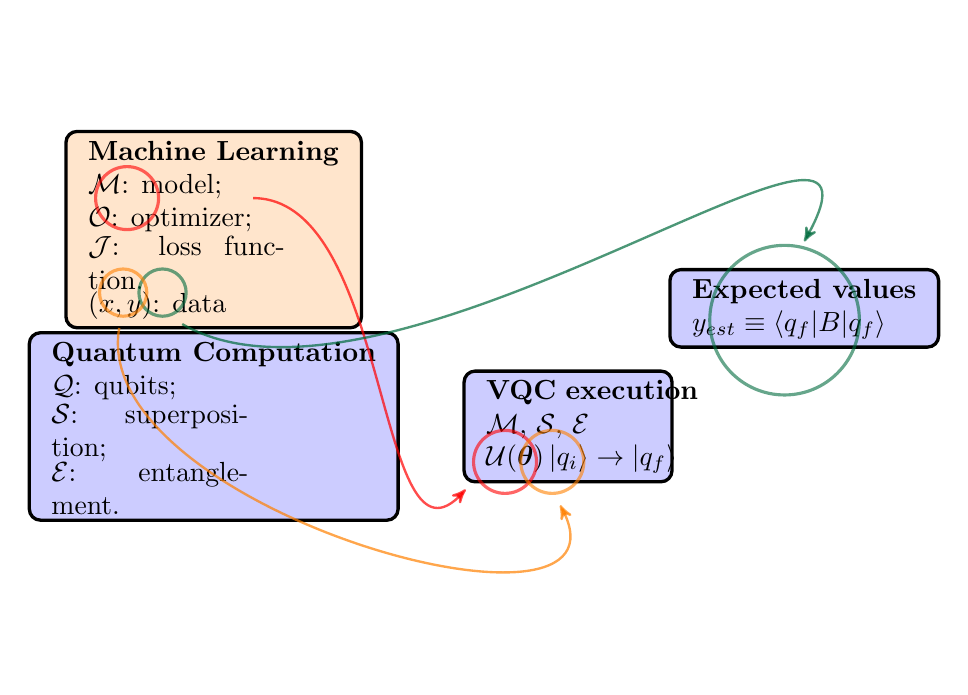
\begin{tikzpicture}[->,>=stealth']

 \node[state, fill=orange!20] (ML) 
 {\begin{tabular}{l}
 \textbf{Machine Learning}\\ 
 \parbox{2.5cm}{$\mathcal{M}$: model;}\\
 \parbox{2.5cm}{$\mathcal{O}$: optimizer;}\\
 \parbox{2.5cm}{$\mathcal{J}$: loss function.}\\
 \parbox{2.5cm}{$(x, y)$: data}
  \end{tabular}
  };
  
  \node[state,
  below of = ML,
  yshift=-1.5cm, fill=blue!20] (QC) 
 {\begin{tabular}{l}
 \textbf{Quantum Computation}\\ 
 \parbox{2.5cm}{$\mathcal{Q}$: qubits;} \\
 \parbox{2.5cm}{$\mathcal{S}$: superposition;}\\
 \parbox{2.5cm}{$\mathcal{E}$: entanglement.}
  \end{tabular}
  };
  
 
 \node[state,
    right of=QC,
    yshift=0cm,
    anchor=center,
    node distance=4.5cm, 	
    text width=2.5cm, fill=blue!20] (VQC) 
 {%
 \begin{tabular}{l}
  \textbf{VQC execution}\\
  $\mathcal{M}$, $\mathcal{S}$, $\mathcal{E}$ \\
  \parbox{2.8cm}{$\mathcal{U}(\bm{\theta})\ket{q_i} \to \ket{q_f}$}
 \end{tabular}
 };
 
\node[state,
  right of = VQC,
  node distance = 3cm,
  yshift=1.5cm, fill=blue!20] (NSHOT) 
 {\begin{tabular}{l}
 \textbf{Expected values}\\ 
 $y_{est} \equiv \braket{q_f|B|q_f}$
  \end{tabular}
  };

  
 \draw[line width=0.3mm, red, opacity = 0.7] (0.5, 0.4)  to[out=0, in=230] (3.2, -3.3);
 \draw[line width=0.3mm, orange, opacity = 0.7] (-1.2, -1.25)  to[out=260, in=300] (4.4, -3.5);
 \draw[line width=0.3mm, cadmiumgreen, opacity = 0.7] (-0.4, -1.2)  to[out=330, in=60] (7.5, -0.15);
  
 
 \draw[red, line width=0.4mm, opacity = 0.6] (3.7,-2.95) circle (0.4 cm);
 \draw[red, line width=0.4mm, opacity = 0.6] (-1.1, 0.4) circle (0.4 cm);
 \draw[cadmiumgreen, line width=0.4mm, opacity = 0.6] (-0.65,-0.8) circle (0.3 cm);
 \draw[cadmiumgreen, line width=0.4mm, opacity = 0.6] (7.25,-1.15) circle (0.95 cm);
 \draw[orange, line width=0.4mm, opacity = 0.6] (4.3,-2.95) circle (0.4 cm);
 \draw[orange, line width=0.4mm, opacity = 0.6] (-1.15,-0.8) circle (0.3 cm);


\end{tikzpicture}
\end{frame}

% SLIDE 5 QML

\begin{frame}{Quantum Machine Learning!}

\vspace{0.25cm}
\begin{tikzpicture}[->,>=stealth']


 \node[state, fill=orange!20] (ML) 
 {\begin{tabular}{l}
 \textbf{Machine Learning}\\ 
 \parbox{2.5cm}{$\mathcal{M}$: model;}\\
 \parbox{2.5cm}{$\mathcal{O}$: optimizer;}\\
 \parbox{2.5cm}{$\mathcal{J}$: loss function.}\\
 \parbox{2.5cm}{$(x, y)$: data}
  \end{tabular}
  };
  
  \node[state,
  below of = ML,
  yshift=-1.5cm, fill=blue!20] (QC) 
 {\begin{tabular}{l}
 \textbf{Quantum Computation}\\ 
 \parbox{2.5cm}{$\mathcal{Q}$: qubits;} \\
 \parbox{2.5cm}{$\mathcal{S}$: superposition;}\\
 \parbox{2.5cm}{$\mathcal{E}$: entanglement.}
  \end{tabular}
  };
  

 \node[state,   
  text width=3cm, 
  yshift=1.5cm, 
  right of=ML, 	
  node distance=4cm, 
  anchor=center, fill=green!20] (OPT) 
 {%
 \begin{tabular}{l} 	% content
  \textbf{Optimizer $\mathcal{O}$}  \\
  \faCode\,\, hybrid-strategy?\\
  \faCogs\,\, on hardware?
 \end{tabular}
 };
 
 \node[state,
    right of=QC,
    yshift=0cm,
    anchor=center,
    node distance=4.5cm, 	
    text width=2.5cm, fill=blue!20] (VQC) 
 {%
 \begin{tabular}{l}
  \textbf{VQC execution}\\
  $\mathcal{M}$, $\mathcal{S}$, $\mathcal{E}$ \\
  \parbox{2.8cm}{$\mathcal{U}(\bm{\theta})\ket{q_i} \to \ket{q_f}$}
 \end{tabular}
 };
 
\node[state,
  right of = VQC,
  node distance = 3cm,
  yshift=1.5cm, fill=blue!20] (NSHOT) 
 {\begin{tabular}{l}
 \textbf{Expected values}\\ 
 $y_{est} \equiv \braket{q_f|B|q_f}$
  \end{tabular}
  };
  
  \node[state,
  above of = NSHOT,
  node distance = 1.5cm,
  yshift=0cm, fill=green!20] (J) 
 {\begin{tabular}{l}
 \textbf{loss function $\mathcal{J}$}\\ 
 $\mathcal{J}(y_{meas}, y_{est})$
  \end{tabular}
  };
  

 \draw[line width=0.3mm] (6, -2.8)  to[out=0, in=250] (7, -1.6);
 \draw[line width=0.3mm] (5.7, -1.1)  to[out=180, in=200] (6, 0.2);
 \draw[line width=0.3mm] (7.5, 1.1)  to[out=90, in=0] (5.7, 1.5);
 \draw[line width=0.6mm, opacity=0.8] (2, 1.6)  to[out=180, in=270] (-0.2, 3.3);
 
 \draw[line width=0.3mm, orange, opacity = 0.0] (-1.2, -1.25)  to[out=260, in=300] (4.4, -3.5);

\end{tikzpicture}
\end{frame}

\section{Full stack algorithms using \texttt{qibo}}

\begin{frame}{\texttt{STEP 0:}  the goal}
\faArrowCircleRight\,\, Let's consider a sample of data $\{x\}_{k=1}^{N_{\rm data}}$.

\faArrowCircleRight\,\,
We can calculate the Cumulative Density Function (CDF) values $F(x)$,

\faArrowCircleRight\,\, which are related to the Probability
Density Function (PDF) via $\rho(x)=\text{d}F(x)/\text{d}x$.

\begin{figure}
    \includegraphics[width=0.7\textwidth]{figures/pdf_cdf.pdf}
\end{figure}
\end{frame}

\begin{frame}
\begin{itemize}
\end{itemize}
\end{frame}

\begin{frame}{\texttt{STEP 0:} the idea}
\begin{figure}  
\includegraphics[width=0.9\textwidth]{figures/pdf_est.png}
\end{figure}
\end{frame}

\begin{frame}[fragile]{Fit CDF with Adiabatic Evolution (AE) \hfill \faTerminal}

\faArrowCircleRight\,\, Given a sample $\{x\}$ and calculated its CDF values $F(x)$:
\pause
\begin{itemize}[noitemsep]
\item[\faChain] we select two hamiltonians $H_0$ and $H_1$ such that a target observable
has energy $E=0$ and $E=1$ respectively on $H_0$ and $H_1$ ground states;
\pause
\item[\faChain] we map $(x, F)\to(\tau, E)$.
\end{itemize}

\pause
\begin{tcolorbox}[colback=amethyst!20, title=Training the evolution]
\begin{itemize}[noitemsep]
\pause
\item[1.] we run the evolution with random initial $\bm{\theta_0}$ into the scheduling;
\pause
\item[2.] we track the energy of a Pauli Z during the evolution;
\pause
\item[3.] we calculate a loss function $J_{\rm mse}$:
         $$ J_{\rm mse} = \sum_{k=1}^{N_{\rm sample}} \bigl[ E(\tau_k) - F(x_k) \bigr]^2; $$
\pause
\item[4.] we choose an optimizer to find $\bm{\theta}_{\rm best}$ which minimizes $J_{\rm mse}$.
\end{itemize} 
\end{tcolorbox}

\end{frame}


\begin{frame}[fragile]{A toy example with \texttt{nqubits=1} - starting point \hfill \faTerminal}
\faArrowCircleRight\,\, \texttt{nparams=20}, \texttt{dt=0.1}, \texttt{final\_time=50}
, \texttt{target\_loss=None}
\begin{figure}
    \includegraphics[width=1\textwidth]{figures/ev0.pdf}
\end{figure}
\end{frame}

\begin{frame}[fragile]{A toy example - until $J_{\rm MSE}=10^{-1}$}
\faArrowCircleRight\,\, \texttt{nparams=20}, \texttt{dt=0.1}, \texttt{final\_time=50}
, \texttt{target\_loss=1e-1}
\begin{figure}
    \includegraphics[width=1\textwidth]{figures/ev1.pdf}
\end{figure}
\end{frame}

\begin{frame}[fragile]{A toy example - until $J_{\rm MSE}=10^{-2}$ \hfill \faTerminal}
\faArrowCircleRight\,\, \texttt{nparams=20}, \texttt{dt=0.1}, \texttt{final\_time=50}
, \texttt{target\_loss=1e-2}
\begin{figure}
    \includegraphics[width=1\textwidth]{figures/ev2.pdf}
\end{figure}
\end{frame}

\begin{frame}[fragile]{A toy example - ending at $J_{\rm MSE}=10^{-4}$ \hfill \faTerminal}
\faArrowCircleRight\,\, \texttt{nparams=20}, \texttt{dt=0.1}, \texttt{final\_time=50}
, \texttt{target\_loss=1e-4}
\begin{figure}
    \includegraphics[width=1\textwidth]{figures/ev3.pdf}
\end{figure}
\end{frame} 

\begin{frame}{From $\{H_{\rm ad}\}$ to a derivable circuit $\mathcal{C}_R$ \hfill \faTerminal}
\faArrowCircleRight\,\, Firstly, we did some calculations and approximations in order to:
\pause
\begin{itemize}[noitemsep]
\item[1.] translate the Hamiltonians' sequence into a single unitary:
$$\prod_{j=1}^{n} e^{-i H_{j}\text{d}t} \to \mathcal{U}(t);$$
\pause 
\item[2.] translate this unitary in a sequence of rotational gates:
$$ \mathcal{U}(t) = R_z(\theta_1)R_x(\theta_2)R_z(\theta_3) \qquad \text{with}\,\, \theta_i \equiv \theta_i(t).$$
\end{itemize}
\pause 
\faArrowCircleRight\,\, Then, we derivate the expected values using parameter shift rule
and chain rule.
\pause 
\begin{multicols}{2}
\begin{figure}
    \includegraphics[width=0.5\textwidth]{figures/PDF_gamma_25_20_200000.pdf}
\end{figure}
\begin{figure}
    \includegraphics[width=0.5\textwidth]{figures/PDF_gauss_30_20_200000.pdf}
\end{figure}
\end{multicols}
\end{frame}

\begin{frame}{\texttt{tii1q\_b1} \hfill \faCogs}
\begin{figure}
    \includegraphics[width=0.9\textwidth]{figures/mit_report_1q.pdf}
    \caption{$N_{\rm runs}=10$ evaluations of CDF predictions for $N_{\rm data}=25$ 
    using $N_{\rm shots}=1000$.}
\end{figure}
\end{frame}

\begin{frame}{Ball to \texttt{qw5q\_gold} \hfill \faCogs}
\begin{figure}
    \includegraphics[width=0.95\textwidth]{figures/5q_hardware.pdf}
    \caption{$N_{\rm runs}=10$ evaluations of CDF predictions for $N_{\rm data}=25$ 
    using $N_{\rm shots}=1000$ and each qubit of \texttt{qw5q\_gold}.}
\end{figure}
\end{frame}


\begin{frame}{The importance of the \texttt{qiboteam}}
\faArrowCircleRight\,\, These first results open several questions:
\pause
\begin{itemize}[noitemsep]
    \item[\footnotesize\faSquare] are these errors compatible with transmon SoA?
    \pause
    \item[\footnotesize\faSquare] which relationship between my results' error and hardware ones?
    \pause
    \item[\footnotesize\faSquare] where are the execution time bottlenecks?
    \pause
    \item[\footnotesize\faSquare] what if we train the entire process on the hardware?
    \pause
    \item[\footnotesize\faSquare] what if we apply error mitigation on predictions?
    \pause
    \item[\footnotesize\faSquare] what if we apply real-time error mitigation?
    \pause
\end{itemize}
\begin{figure}
    \includegraphics[width=0.8 \textwidth]{figures/mr_research.png}
\end{figure}
\end{frame}

\begin{frame}{The importance of the \texttt{qiboteam}}
\faArrowCircleRight\,\, These first results open several questions:
\begin{itemize}[noitemsep]
    \item[\footnotesize\faSquare] are these errors compatible with transmon SoA?
    \item[\footnotesize\faSquare] which relationship between my results' error and hardware ones?
    \item[\footnotesize\faSquare] where are the execution time bottlenecks?
    \item[\footnotesize\faSquare] \textcolor{amethyst}{\textbf{what if we train 
    the entire process on the hardware?}}
    \item[\footnotesize\faSquare] what if we apply error mitigation on predictions?
    \item[\footnotesize\faSquare] what if we apply real-time error mitigation?
\end{itemize}
\begin{figure}
    \includegraphics[width=0.8 \textwidth]{figures/mr_research.png}
\end{figure}
\end{frame}


\begin{frame}{A QML training on \texttt{tii1q\_b1}}
\faArrowCircleRight\,\,Following \href{https://arxiv.org/abs/1907.02085}{\textit{Pérez-Salinas et al.}} 
procedure, we can build a \textit{universal quantum regressor}
for approximating $y=f(x)$. 
\pause 

\faArrowCircleRight\,\, The model can be:
\pause
    \begin{figure}  
    \includegraphics[width=0.85\textwidth]{figures/qpdf.png}
    \caption{Here $\xi_A= \theta_1x+\theta_2$ and $\xi_B = \theta_3x + \theta_4$.}
    \end{figure}
\pause
\faArrowCircleRight\,\, and then use some $E[\hat{O}]$ as predictor:
\begin{equation}
y_{pred} = \braket{0 | \mathcal{C}^{\dagger} (x; \bm{\theta}) \hat{O} \,
\mathcal{C} (x; \bm{\theta}) | 0}.
\end{equation}
\pause
\faArrowCircleRight\,\, Using the parameter-shift rule, we can perform a gradient descent on \texttt{tii1q\_b1}.
\end{frame}

\begin{frame}{Running on \texttt{tii1q\_b1}\hfill \faCogs}

    \begin{figure}  
    \includegraphics[width=1\textwidth]{figures/qpu1.pdf}
    \caption{Batch Gradient Descent on the hardware, with gradients evaluated 
    via Parameter-Shift Rule. We take $100$ points $\{x_j\}$ in the range $[-1,1]$ and we make 
    $100$ predictions for each $x_j$. Mean and standard deviation are used for 
    determining the estimations and the confidend belt.}
    \end{figure}

\end{frame}

\begin{frame}{Normalised results \hfill \faCogs}

    \begin{figure}  
    \includegraphics[width=1\textwidth]{figures/ratio_plot.pdf}
    \caption{Normalised results of the SGD (green line) compared with true law 
    and a genetic optimizer (red line).}
    \end{figure}

    \pause
    \begin{itemize}[noitemsep]
    \item[\faThumbsUp] the full-stack framework works! comparable with a genetic algorithm;
    \pause
    \item[\faThumbsDown] we can tackle only easy problems: it is slow;
    \pause
    \item[\faMehO] no mitigation: have been the errors absorbed into the optimization?
    \end{itemize}

\end{frame}

\begin{frame}{The importance of the \texttt{qiboteam}}
\faArrowCircleRight\,\, These first results open several questions:
\begin{itemize}[noitemsep]
    \item[\footnotesize\faSquare] are these errors compatible with transmon SoA?
    \item[\footnotesize\faSquare] which relationship between my results' error and hardware ones?
    \item[\footnotesize\faSquare] where are the execution time bottlenecks?
    \item[\footnotesize\faSquare] what if we train 
    the entire process on the hardware?
    \item[\footnotesize\faSquare] \textcolor{amethyst}{\textbf{what if we apply 
    error mitigation on predictions?}}
    \item[\footnotesize\faSquare] what if we apply real-time error mitigation?
\end{itemize}
\begin{figure}
    \includegraphics[width=0.8 \textwidth]{figures/mr_research.png}
\end{figure}
\end{frame}

\begin{frame}{Mitigated prediction of the PDF}
    \begin{figure}
    \includegraphics[width=0.5\textwidth]{figures/no_mit.jpeg}%
    \includegraphics[width=0.5\textwidth]{figures/mit.jpeg}%
    \caption{Predictions of a sinus function performed on \texttt{tii1q\_b1} without
    and with CDR mitigation.}
    \end{figure}
\faArrowCircleRight\,\, These results open to new questions!
\begin{itemize}[noitemsep]
\pause
    \item[\scriptsize\faSquare] can QEM help the training with a faster convergence?
\pause
    \item[\scriptsize\faSquare] what's the right balance between error absorption and QEM?
\pause
    \item[\scriptsize\faSquare] can we train the unmitigated hardware to be self-resistent?
\end{itemize}
\end{frame}

\begin{frame}{The importance of the \texttt{qiboteam}}
\faArrowCircleRight\,\, These first results open several questions:
\begin{itemize}[noitemsep]
    \item[\footnotesize\faSquare] are these errors compatible with transmon SoA?
    \item[\footnotesize\faSquare] which relationship between my results' error and hardware ones?
    \item[\footnotesize\faSquare] where are the execution time bottlenecks?
    \item[\footnotesize\faSquare] what if we train 
    the entire process on the hardware?
    \item[\footnotesize\faSquare] what if we apply error mitigation on predictions?
    \item[\footnotesize\faSquare] \textcolor{amethyst}{\textbf{what if we apply real-time error mitigation?}}
\end{itemize}
\begin{figure}
    \includegraphics[width=0.8 \textwidth]{figures/mr_research.png}
\end{figure}
\end{frame}

\begin{frame}{Real-time error mitigation \hfill \faTerminal}
\faArrowCircleRight\,\, We want to reproduce the $u$ quark PDF fit of \href{https://arxiv.org/abs/2011.13934}{\textit{Pérez-Salinas et al}}.

\pause
\faArrowCircleRight\,\, We apply error mitigation techniques\footnote{
    We used Zero Noise Extrapolation (ZNE) and Clifford Data Regresssion (CDR).
} during
a QML training! 
\pause
    \begin{figure}
    \includegraphics[height=3cm, width=0.33\textwidth]{figures/exact.pdf}%
    \includegraphics[height=3cm, width=0.33\textwidth]{figures/noisy.pdf}%
    \includegraphics[height=3cm, width=0.33\textwidth]{figures/mitigated.pdf}%
    \caption{PDF fit performed with different levels of noisy simulation. 
    From left to right, exact simulation, noisy simulation, noisy simulation 
    applying error mitigation to the predictions.}
    \end{figure}
\pause
\faArrowCircleRight\,\, \textbf{\textcolor{amethyst}{But on the hardware?}}
\end{frame}

\begin{frame}{Run on \texttt{tii1q\_b1} \hfill \faCogs}
\begin{figure}
    \includegraphics[width=0.9\textwidth]{figures/bench-platforms.pdf}
    \caption{Full training is here performed on \texttt{tii1q\_b1}. We then used 
    the $\bm{\theta}_{\rm best}$ to make statistics on 30 points and 30 runs with
    simulation (blue line) and on the device (red line).} 
\end{figure}
\end{frame}



\section{Conclusions}


\begin{frame}{\texttt{qibo} as research network!}
\pause

\faArrowCircleRight\,\, The \texttt{qibo} environment is perfect for this kind of research, because
\begin{itemize}[noitemsep]
\pause
    \item[\faCogs] we have resources deputed to the research;
\pause
    \item[\faChild] we are a fully connected research network.
\end{itemize}
\pause

\faArrowCircleRight\,\, Moreover, \texttt{qibo} is growing as international environment:
\pause

\begin{figure}
    \includegraphics[width=1 \textwidth]{figures/network_cern.png}
\end{figure}
\end{frame}

\begin{frame}{Thanks!}
\begin{figure}
    \includegraphics[width=1 \textwidth]{figures/mr_research.png}
\end{figure}
\end{frame}


\end{document}
